\documentclass{article}
\usepackage[
        a4paper,
        left=3cm,
        right=3cm,
        top=3cm,
        bottom=4cm,
]{geometry}
\usepackage{graphicx}
\usepackage{caption}
\usepackage{enumerate}
\usepackage{subcaption}
\usepackage[procnames]{listings}
\usepackage{color}
\usepackage{amsmath}
\usepackage{hyperref}
\usepackage{float}
\title{Lab Assignement 0}
\date{\today}
\author{
	Karamoulas Eleftherios - S3261859\\
	Tzafos Panagiotis - S3302148\\
}

\begin{document}
\maketitle
\section{Answers for Lab 0}
\begin{enumerate}
\item
After our experiments, having conducted a parameter sweep of the factors we came to the conclusion that when we conduct a parameter sweep for Rin low values, the result is spare spikes and when the value gets increased, the spikes occur more often until Rin reaches a high value that turns v(n) to zero and in this case we have very few spikes. When we sweep tau, because he is the divisor in our equation, low values of tau give frequent spikes and the increase of tau has as a result to reach a point where we have no spikes. Finally, the sweep of theta, as it is the factor that limits our v(n), when it is about to become zero again, has as a result, small values of theta make the spike occurency higher and while theta gets increased, the frequency of spikes drops down.
\item ~
\begin{figure}[H]
    \centering
    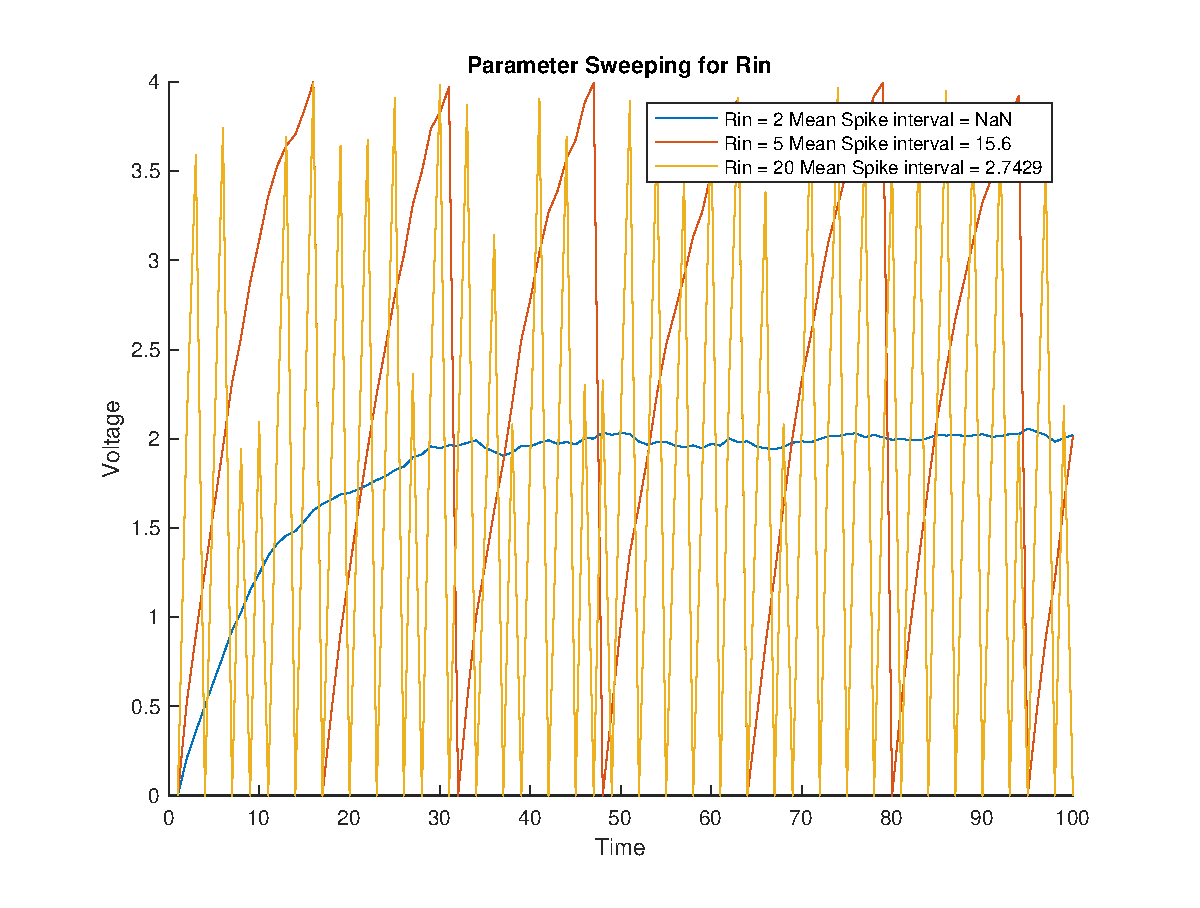
\includegraphics[width=0.7\textwidth]{im/Rin-Sweep.eps}
    \caption{R-sweep}
    \label{fig:plot}
  \end{figure}
  \begin{figure}[H]
    \centering
    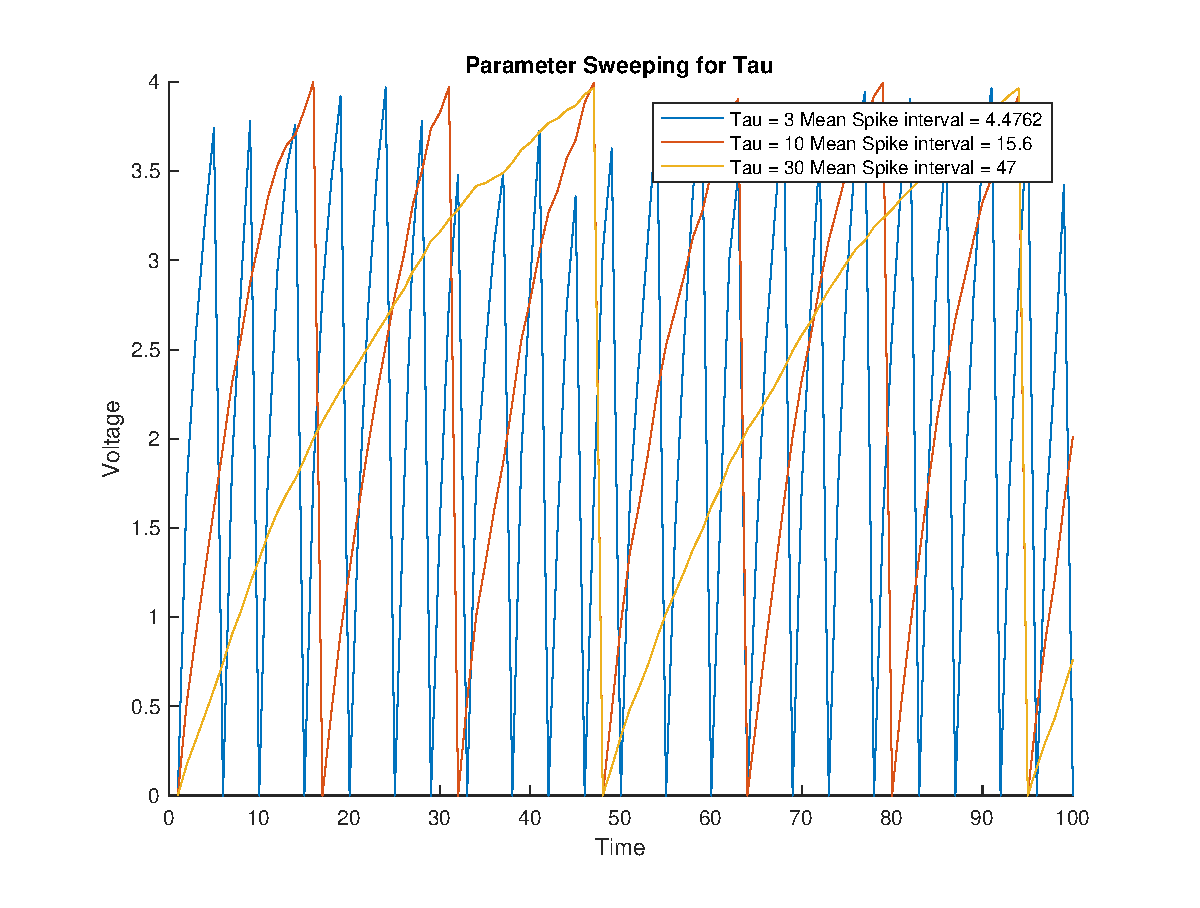
\includegraphics[width=0.7\textwidth]{im/Tau-Sweep.eps}
    \caption{Tau-sweep}
    \label{fig:plot}
  \end{figure}
  \begin{figure}[H]
    \centering
    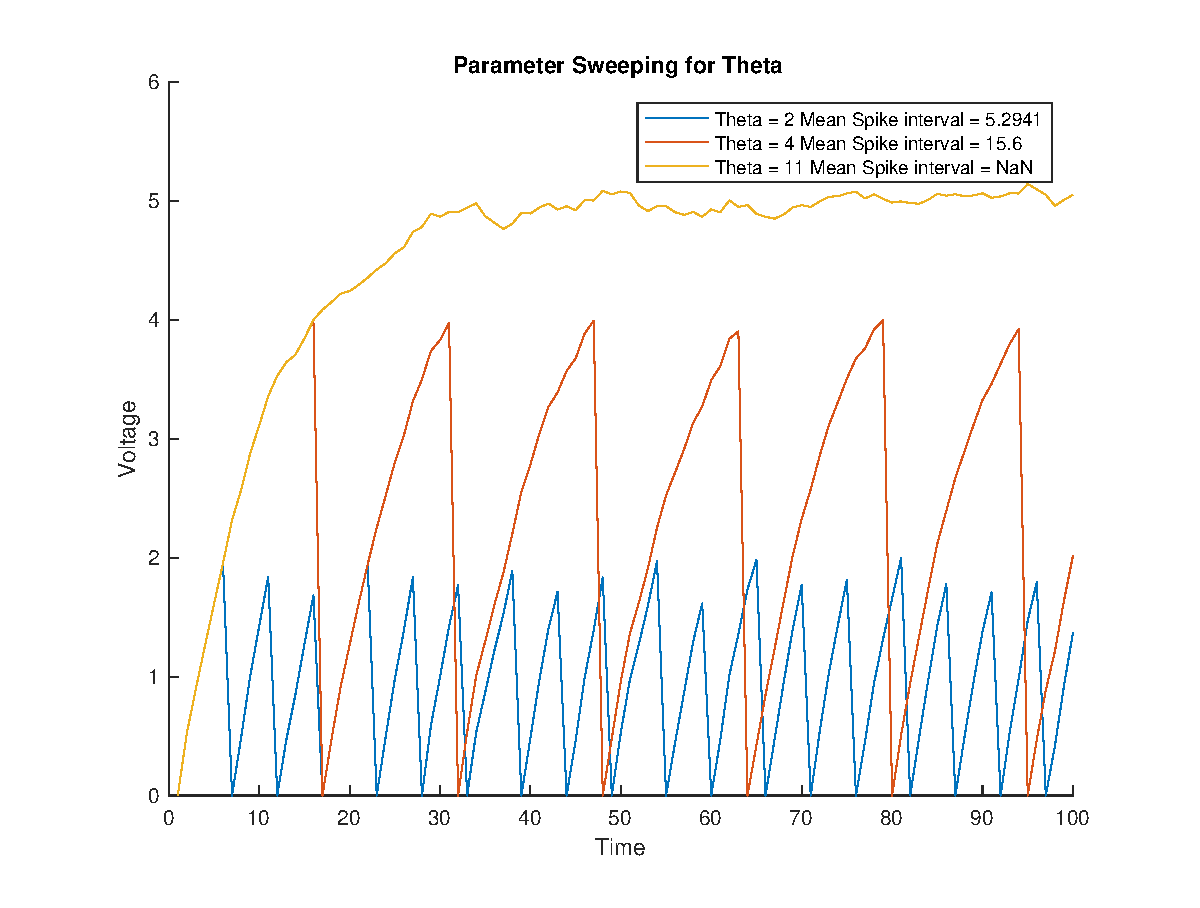
\includegraphics[width=0.7\textwidth]{im/Theta-Sweep.eps}
    \caption{Theta-sweep}
    \label{fig:plot}
  \end{figure}
\item
\lstinputlisting[caption={noisyifneuron.m},label={code:bar}]{src/noisyifneuron.m}
\lstinputlisting[caption={isi.m},label={code:bar}]{src/isi.m}
\end{enumerate}
\end{document}
